\part{监督学习}
监督学习是从标记的训练数据来推断一个功能的机器学习任务。训练数据包括一套训练示例。在监督学习中,每个实例都是由一个输入对象(通常为矢量)和一个期望的输出值(也称为监督信号)组成。监督学习算法是分析该训练数据,并产生一个推断的功能,其可以用于映射出新的实例。一个最佳的方案将允许该算法来正确地决定那些看不见的实例的类标签。这就要求学习算法是在一种“合理”的方式从一种从训练数据到看不见的情况下形成。

当采用了监督学习后,进一步确定目标变量若为离散值(标称量),则采用分类算法进行学习;若为连续值,则采用回归算法进行学习。

\section{分类}
监督学习的分类算法有很多,最简单的k-邻近算法,还有决策树,朴素贝叶斯,逻辑回归,支持向量机,Adaboost算法等。这些算法都有其特性,或多或少的公式推理,我都要去熟悉,学习,加实战。

\subsection{逻辑回归}
逻辑回归(Logistics Regression)是一种通过画出训练样本的决策边界,解决某种数据拟合二分类问题的有效途径。
对于怎样画出决策边界则为此算法核心。
我从逻辑函数(Logistic Function)的由来入手,学习了指数分布族,广义线性模型。

\subsubsection{指数分布簇}

介绍指数分布族(Exponential Family)为下一小节的广义线性模型(GLM)做铺垫。指数分布簇抽象统一形式为:
\begin{equation}
  p(y;\eta)=b(y)exp(\eta^T T(y)-a(\eta))
\end{equation}
其中参数$\eta$是自然常量;$T(y)$充分统计量(通常情况下$T(y)=y$);$a(\eta)$为对数划分函数;
给定三个函数$a(\eta),b(y),T(y)$就能确定一组概率分布;如在给定$\eta$值,便可以确定唯一一个概率分布。
那么有哪些常见分布属于指数分布族:
\begin{enumerate}
  \item 正态分布
  \item 二项分布
  \item 多项式分布
\end{enumerate}

\subsubsection{广义线性模型}
广义线性模型通过对指数分布族内分布进行建模得到响应函数从而得到目标函数,再通过某种最优化的算法(牛顿法/梯度上升法)得到最优系数,从而得到目标连接模型。
构建广义线性模型的步骤为,也就是广义线性模型的形式化定义为:
\begin{enumerate}
  \item $y|x;\theta \sim ExponentialFamily(\eta)$ \\即就是在给定$x,\theta$后,$y$满足的概率分布是以$\eta$为自然常数的指数分布族的一员。
  \item 给定x,输出~$h(x)=E[T(y)|x]$~即目标得到y的期望值。
  \item 最后令~$\eta=\theta^Tx$~(线性模型) 得到目标连接函数。
\end{enumerate}

现在以Bernoulli分布为例,构建广义线性模型,得到逻辑函数(也叫Sigmoid函数)。
现知道二项分布的概率密度函数为:
\begin{equation}\nonumber
\begin{split}
  p(y;\phi)&= \phi^y(1-\phi)^{1-y}\\
           &= exp~(yln\phi+(1-y)ln(1-\phi))\\
           &= exp~((ln(\frac{\phi}{1-\phi}))y+ln(1-\phi))
\end{split}
\end{equation}
对照指数分布族的抽象式(1)得到(这里~$\eta$~是标量):
\begin{equation}\nonumber
\begin{split}
  \eta   &=ln(\frac{\phi}{1-\phi}) \\
  T(y)   &= y\\
  a(\eta)&= -ln(1-\phi)\\
         &= ~ln(1+e^\eta)\\
  b(y)   &= 1\\
\end{split}
\end{equation}
得到关联函数:
\begin{equation}\nonumber
\begin{split}
  h_\theta(x) &= E(y|x;\theta)\\
              &= \phi~~~ (0-1~distribution's~mean)\\
              &= \frac{1}{1+e^{-\eta}}~~~(link function)\\
              &= \frac{1}{1+e^{-\theta^T x}}
\end{split}
\end{equation}

\subsubsection{理论:利用梯度上升做逻辑回归}
首先知道逻辑函数,所以令:
$$h_\theta(x)=g(\theta^T x)=\frac{1}{e^-\theta^Tx}$$
其中,
$$g(z)=\frac{1}{1+e^{-z}}$$
可以看出当~$z\rightarrow\infty~$时 ,$g(z)\rightarrow1$;当~$z\rightarrow-\infty~$时 ,$g(z)\rightarrow0$;
再令~$x_0=1$~,则:
$$\theta^Tx=\theta_0+\sum_{j=1}^{n}\theta_jx_j$$

$g(z)$~对z求导:
\begin{equation}
\begin{split}
  g'(z) &= \frac{\partial}{\partial z}\frac{1}{1+e^{-z}}\\
        &= \frac{1}{(1+e^{-z})^2}(e^{-z})\\
        &= \frac{1}{1+e^{-z}}\cdot(1-\frac{1}{(1+e^{-z})})\\
        &= g(z)(1-g(z))
\end{split}
\end{equation}

既然逻辑函数值表示概率,则:
\begin{equation}\nonumber
\begin{split}
  P(y=1|x;\theta) &= h_\theta(x)\\
  P(y=0|x;\theta) &= 1-h_\theta(x)
\end{split}
\end{equation}
即就是,
$$P(y|x;\theta)=(h_\theta(x))^y(1-h_\theta(x))^{1-y}$$
之后在对其进行极大似然估计:
\begin{equation}\nonumber
\begin{split}
  L(\theta) &= p(\overrightarrow{y}|X;\theta)\\
            &= \prod_{i=1}^{m}p(y^{(i)}|x^{(i)};\theta)\\
            &= \prod_{i=1}^{m}(h_\theta(x^{(i)}))^{y^{(i)}}(1-h_\theta(x^{(i)})^{1-y^{(i)}}\\
  l(\theta) &= ln L(\theta)\\
            &= \sum_{i=1}^{m}y^{(i)}lnh(x^{(i)})+(1-y^{(i)})ln(1-h(x^{(i)}))
\end{split}
\end{equation}
最终为了得到最大的~$l(\theta)$~,利用一种最优化算法梯度上升来求取,要求梯度,即求导:
\begin{equation}\nonumber
\begin{split}
  \frac{\partial}{\partial\theta_j}l(\theta) &= ( y\frac{1}{g(\theta^Tx)}-(1-y)\frac{1}{1-g(\theta^Tx)})\frac{\partial}{\partial\theta_j}g(\theta^Tx)\\
            &= ( y\frac{1}{g(\theta^Tx)}-(1-y)\frac{1}{1-g(\theta^Tx)})g(\theta^Tx)(1-g(\theta^Tx))\frac{\partial}{\partial\theta_j}\theta^Tx\\
            &= (y(1-g(\theta^Tx))-(1-y)g(\theta^Tx))x_j\\
            &= (y-h_\theta(x))x_j
\end{split}
\end{equation}
得到梯度后,再利用随机梯度上升(stochastic gradient ascent)迭代更新系数:
\begin{equation}\nonumber
\begin{split}
  \theta_j ~:=\theta_j+\alpha(y^{(i)}-h_\theta(x^{(i)}))x_j^{(i)}
\end{split}
\end{equation}

\subsubsection{实现:利用梯度上升做逻辑回归}
实战中利用的是梯度上升的最优化算法,逻辑回归就是利用最优化算法来训练出一个非线性函数用于分类。期间核心是利用最优化算法来寻找最佳拟合参数。
逻辑回归的优点是计算代价不高,易于理解与实现;其缺点是容易欠拟合,分类精度不高;适用数据类型是数值型与标称型数据。
逻辑回归的一般过程为:
\begin{enumerate}
  \item 收集数据:任意方法收集。
  \item 准备数据:最好为结构化数据。
  \item 分析数据:任意方法分析数据。
  \item 训练数据:大部分时间用来训练数据。
  \item 测试算法:测试会很快完成。
  \item 使用算法:输入数据,转结构化,进行回归计算,判定类别。
\end{enumerate}

\noindent\textbf{梯度上升找最佳参数~$\theta$~}\par
梯度上升算法的迭代公式如下,利用python实现。
\begin{equation}\nonumber
\begin{split}
  w := w +\alpha\nabla_wf(w)
\end{split}
\end{equation}

\noindent程序核心函数代码:
\begin{lstlisting}
def sigmoid(inX):
    return 1.0/(1+exp(-inX))

def gradAscent(dataMatIn, classLabels):
    dataMatrix = mat(dataMatIn)             #convert to NumPy matrix
    labelMat = mat(classLabels).transpose() #convert to NumPy matrix
    m,n = shape(dataMatrix)
    alpha = 0.001
    maxCycles = 600                         #Number of iterations
    weights = ones((n,1))
    for k in range(maxCycles):              #heavy on matrix operations
        h = sigmoid(dataMatrix*weights)     #matrix mult
        #print(dataMatrix*weights)          #$\eta$
        error = (labelMat - h)              #vector subtraction
        weights = weights + alpha * dataMatrix.transpose()* error #matrix mult
    return weights

def plotBestFit(weights):
    import matplotlib.pyplot as plt
    dataMat,labelMat=loadDataSet()
    dataArr = array(dataMat)
    n = shape(dataArr)[0]
    xcord1 = []; ycord1 = []
    xcord2 = []; ycord2 = []
    for i in range(n):
        if int(labelMat[i])== 1:
            xcord1.append(dataArr[i,1]); ycord1.append(dataArr[i,2])
        else:
            xcord2.append(dataArr[i,1]); ycord2.append(dataArr[i,2])
    fig = plt.figure()
    ax = fig.add_subplot(111)
    ax.scatter(xcord1, ycord1, s=30, c='red', marker='s')
    ax.scatter(xcord2, ycord2, s=30, c='green')
    x = arange(-3.0, 3.0, 0.1)
    y = (-weights[0]-weights[1]*x)/weights[2]
    ax.plot(x, y)
    plt.xlabel('X1'); plt.ylabel('X2');
    plt.show()
    plt.savefig('LogRegres_GradAscent.eps',dpi=2000)
\end{lstlisting}

利用测试数据得到初步的分类结果,并可视化表示结果如下图:
\begin{figure}[!hbt]
  \centering
  \includegraphics[width=0.6\textwidth]{1141.eps}
  \caption{利用梯度上升做逻辑回归的分类结果}
\end{figure}

\noindent分析图1:\\
\indent分类结果相当不错,从图中看上去只有四个点分类错误,但是知道一共需要600次迭代,也就是说至少要有600次的全训练数据的矩阵乘运算。
因此,不能将其作用于真实数据集的主要原因有二:其一时间复杂度缺陷;其二每一次迭代运算都需要作用于全体训练集,不利用扩充训练集。\\
接下来学习的随机梯度上升算法解决上述两类问题。

\noindent\textbf{随机梯度上升找最佳参数~$\theta$~}\par
随机梯度上升算法(Stochastic Gradient Ascent Algorithm)是一个在线学习算法,由于其可以在新样本到来时对分类器进行增量式的更新。与在线学习算法相对应的是,一次处理所有的数据被称为是批处理。\\
而随机梯度上升的迭代公式为:
\begin{equation}\nonumber
\begin{split}
  \theta_j ~:&=\theta_j+\alpha(y^{(i)}-h_\theta(x^{(i)}))x_j^{(i)}~~~~~~one~coefficient\\
  \Longrightarrow
  w :&= w+\alpha(y^{(i)}-h_\theta(x^{(i)}))x^{(i)}~~~~~~all~coefficient
\end{split}
\end{equation}

\noindent程序核心函数代码:
\begin{lstlisting}
def stocGradAscent0(dataMatrix, classLabels):
    m,n = shape(dataMatrix)
    # print (m,n)
    alpha = 0.01
    weights = ones(n)   #initialize to all ones
    for i in range(m):
        h = sigmoid(sum(dataMatrix[i]*weights))
        error = classLabels[i] - h
        weights = weights + alpha * error * dataMatrix[i] #Non matrix operation
    return weights
\end{lstlisting}

还是利用之前的测试数据得到初步的分类结果,并可视化表示结果如下图:
\begin{figure}[!hbt]
  \centering
  \includegraphics[width=0.6\textwidth]{1142.eps}
  \caption{利用随机梯度上升做逻辑回归的分类结果,并非最佳分类线}
\end{figure}

首先看回归系数与迭代次数的关系图:
\begin{figure}[!hbt]
  \centering
  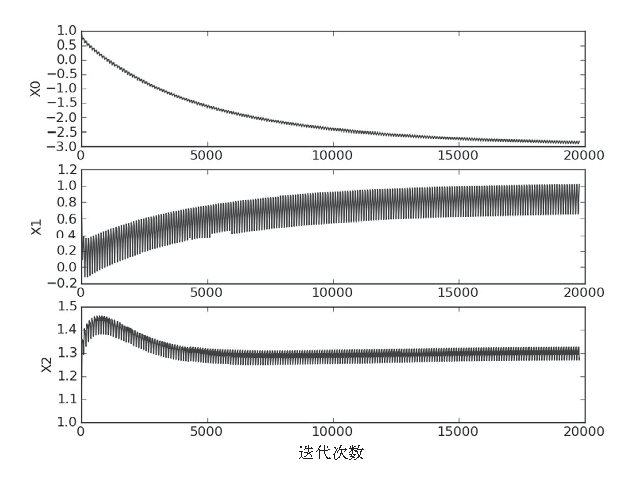
\includegraphics[width=0.65\textwidth]{1143.eps}
  \caption{回归系数与迭代次数的关系图}
\end{figure}

\noindent分析:\\
\indent分类器分错了三分之一的样本,但是只进行了类似于上节批量梯度下降的一次矩阵运算,所以结果并不公平。\\
此外看到,存在一些不能正确分类的样本点,导致了在每次迭代的时,会引发系数的剧烈变化。
于是期望算法能避免来回波动,从而收敛到某个值;以及收敛的速度也应加快。
只要对其进行改进,效果则立竿见影。\\


\noindent\textbf{改进的随机梯度上升找最佳参数~$\theta$~}\par
\noindent程序核心函数代码:
\begin{lstlisting}
def stocGradAscent1(dataMatrix, classLabels, numIter=150):
    m,n = shape(dataMatrix)
    weights = ones(n)   #initialize to all ones
    for j in range(numIter):
        dataIndex = list(range(m))
        for i in range(m):
            alpha = 4/(1.0+j+i)+0.0001    #alpha decreases with iteration, does not
            randIndex = int(random.uniform(0,len(dataIndex)))#go to 0 because of the constant
            h = sigmoid(sum(dataMatrix[randIndex]*weights))
            error = classLabels[randIndex] - h
            weights = weights + alpha * error * dataMatrix[randIndex]
            del(dataIndex[randIndex])
            # print(dataIndex)
    return weights
\end{lstlisting}


还是利用之前的测试数据得到初步的分类结果,并可视化表示结果如下图:
\begin{figure}[!htb]
  \centering
  \includegraphics[width=0.6\textwidth]{1144.eps}
  \caption{利用改进的随机梯度上升做逻辑回归的分类结果}
\end{figure}


\noindent 算法参数分析:\\
\indent1.设置动态步长~$\alpha$~,缓解上节中数据的波动或者高频波动,比固定的$~\alpha~$收敛速度更快。当$~j<<max(i)~$时,$\alpha~$就不是严格下降,
避免参数的严格下降也常见于模拟退火算法等其他优化算法当中。\\
\indent2.训练样本随机选取更新回归系数,为了减少上节的周期性波动。

\begin{figure}[!htb]
  \centering
  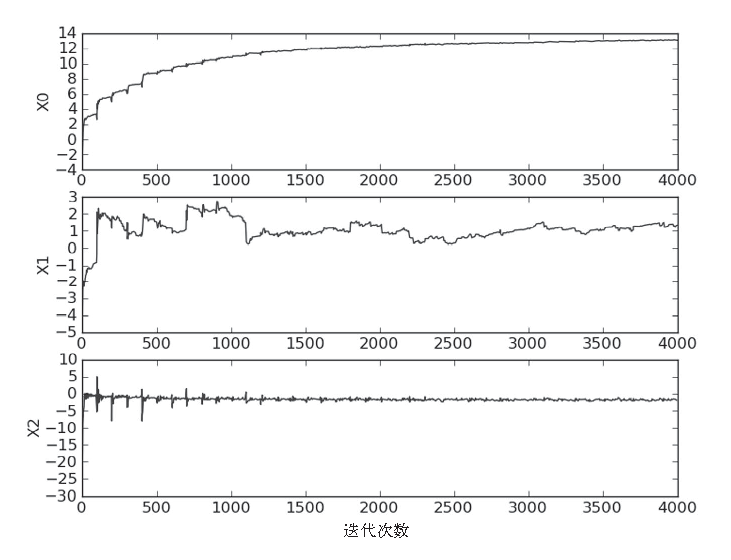
\includegraphics[width=0.65\textwidth]{1145.eps}
  \caption{改进算法后回归系数与迭代次数关系图}
\end{figure}

\noindent分析:\\
\indent改进的随机梯度下降优化算法与批量梯度下降优化算法相比,分类结果的效果差不多,但是所使用的计算量更少,
再利用小量的训练集时间差别不大,但是如果处理数以十亿计的训练样本和成千上万的特征时,两者的优越性则显露无疑。

\subsubsection{实战:利用逻辑回归,从疝气病症预测病马的死亡率}
将使用Logistic回归来预测患有疝病的马的存活问题。
这里数据包含368个样本,与28个特征;但有的指标比较主观,有的指标难以测量,例如马的疼痛级别。

另外,该数据有30\%的数据缺失用0填充,一条样本只有21个feature和1个label。\\
实战的步骤:
\begin{enumerate}
  \item 收集数据:给定数据文件。
  \item 准备数据:用python解析文本文件并填充缺失值。
  \item 分析数据:可视化并观察数据。
  \item 训练算法:使用优化算法,找到最佳的系数。
  \item 测试算法:观测错误率,回退调参,得到更好的回归系数。
  \item 使用算法:预测病马死亡率。
\end{enumerate}

\noindent\textbf{准备数据}\par
数据无价,数据中的缺失值,不能轻易的丢弃掉,有时也不能轻易的重新获取,必须采用一些方法来处理数据中的缺失值。这里采用的是使用特殊值来填充,用0填充,其对结果的预测不具有任何倾向性,因为$sigmoid(0)=0.5$。
\begin{enumerate}
  \item 使用特征均值填补缺失值。
  \item 使用特殊值来填补缺失值,如-1。
  \item 忽略有缺失值的样本。
  \item 使用相似样本的均值填补缺失值。
  \item 使用另外的机器学习算法预测缺失值。
\end{enumerate}

\noindent\textbf{测试算法}\par
将训练集中的数据进行逻辑回归分析,得出回归系数向量。在与特征向量相乘输入到sigmoid函数当中,结果大于0.5,预测为1;否则为0。\\
\noindent程序核心函数代码:
\begin{lstlisting}
def sigmoid(inX):
    if inX<-700:
        inX = -700    #avoid exp_function overflow
    return 1.0/(1+exp(-inX))

def stocGradAscent1(dataMatrix, classLabels, numIter=150):
    m,n = shape(dataMatrix)
    weights = ones(n)   #initialize to all ones
    for j in range(numIter):
        dataIndex = list(range(m))
        for i in range(m):
            alpha = 4/(1.0+j+i)+0.0001    #apha decreases with iteration, does not
            randIndex = int(random.uniform(0,len(dataIndex)))#go to 0 because of the constant
            h = sigmoid(sum(dataMatrix[randIndex]*weights))
            error = classLabels[randIndex] - h
            weights = weights + alpha * error * dataMatrix[randIndex]
            del(dataIndex[randIndex])
    # print("weight=",weights)
    return weights

def classifyVector(inX, weights):
    prob = sigmoid(sum(inX*weights))
    if prob > 0.5: return 1.0
    else: return 0.0

def colicTest():
    frTrain = open('horseColicTraining.txt'); frTest = open('horseColicTest.txt')
    trainingSet = []; trainingLabels = []
    for line in frTrain.readlines():
        currLine = line.strip().split('\t')
        lineArr =[]
        for i in range(21):
            lineArr.append(float(currLine[i]))
        trainingSet.append(lineArr)
        trainingLabels.append(float(currLine[21]))
    trainWeights = stocGradAscent1(array(trainingSet), trainingLabels, 1000)
    errorCount = 0; numTestVec = 0.0
    for line in frTest.readlines():
        numTestVec += 1.0
        currLine = line.strip().split('\t')
        lineArr =[]
        for i in range(21):
            lineArr.append(float(currLine[i]))
        if int(classifyVector(array(lineArr), trainWeights))!= int(currLine[21]):
            errorCount += 1
    errorRate = (float(errorCount)/numTestVec)
    print ("the error rate of this test is: %f" % errorRate)
    return errorRate

def multiTest():
    numTests = 10; errorSum=0.0
    for k in range(numTests):
        errorSum += colicTest()
    print ("after %d iterations the average error rate is: %f" % (numTests, errorSum/float(numTests)))
\end{lstlisting}

\noindent\textbf{预测结果}\par
\begin{lstlisting}
the error rate of this test is: 0.343284
the error rate of this test is: 0.328358
the error rate of this test is: 0.283582
the error rate of this test is: 0.298507
the error rate of this test is: 0.417910
the error rate of this test is: 0.417910
the error rate of this test is: 0.298507
the error rate of this test is: 0.358209
the error rate of this test is: 0.313433
the error rate of this test is: 0.343284
after 10 iterations the average error rate is: 0.340299
\end{lstlisting}

利用改进的随机梯度下降算法迭代求得回归系数,最终在作用于测试集,得到预测的平均错误率为34\%。这个结果相对不错,因为有30\%的数据缺失。事实上错误率还可以通过调参往下降。

\subsubsection{小结}
逻辑回归这一章从逻辑函数由来入手,学习了指数分布族,广义线性模型。知道逻辑函数是由bernoulli分布广义线性建模的结果。还给了必要的理论证明。

逻辑回归目的是寻找一个非线性函数Sigmoid的最佳拟合参数,求解过程可以由最优化算法来完成。最常用的就是梯度上升算法,而梯度上升算法可以改进为随机梯度上升算法。

随机梯度上升算法的效果相当,但占用更少的计算机资源。此外,随机梯度上升是一个在线算法,它可以在新的数据到来时就可以完成更新,而不需要重新读取整个数据集来进行批处理运算。

机器学习的一个重要的问题就是如何处理缺失数据。这个问题没有标准答案,取决于实际应用中的需求。现有的解决方案都各自有优缺点。

\newpage



\subsection{高斯判别算法}
\subsubsection{生成学习算法}
逻辑回归或者感知机算法是在给定~x~的情况下直接对$~p(y|x;\theta)~$进行建模。其都是试图做分类边界,来进行分类;
那换个思路就是对各个分类目分别建立模型,最终将新样本输入到各个分类目模型当中去试图分类。

\noindent\textbf{判别学习算法}\par
判别学习算法(discriminative learning algorithm):直接学习$~p(y|x)~$或者是从输入直接映射到输出的方法;逻辑回归与感知机算法就是这一类算法的代表。

\noindent\textbf{生成学习算法}\par
生成学习算法(generative learning algorithm):对$~p(x|y)~$(也包括$~p(y)~$)进行建模。\\
建模方式:\\
输出两类:~~~~$y\in\{0,1\}$\\
$p(x|y=0):$~~~对0类特征进行建模\\
$p(x|y=1):$~~~对1类特征进行建模\\
完成对$~p(x|y)~$,以及$~p(y)~$的建模后。利用~Bayes~公式求得再给定~x~情况下~y~的概率,如下:
\begin{equation}\nonumber
\begin{split}
  &p(y|x)=\frac{p(x|y)p(y)}{p(x)}\\
  p(x)=p(x|y&=1)p(y=1)+p(x|y=0)p(y=0)
\end{split}
\end{equation}
最后再对$~p(x,y)~$进行最大似然估计,得到最佳参数。\\
最终将新样本输入到各个模型中得到概率值,判定类目。\\
事实上。可以不用完全算出概率值,比较不同类目输出结果大小即可。
\begin{equation}\nonumber
\begin{split}
  arg~\mathop{max}_y~p(y|x)&=arg~\mathop{max}_y\frac{p(x|y)p(y)}{p(x)}\\
  &=arg~\mathop{max}_y~p(x|y)p(y)\\
\end{split}
\end{equation}
常见的生成模型有:高斯判别分析,隐马尔可夫模型HMM,朴素贝叶斯模型,高斯混合模型GMM,LDA等。

\subsubsection{多项正太分布}
n维多项分布也称多项高斯分布,均值向量$~\mu\in R^n~$,协方差矩阵$~\Sigma\in R^{n\times n}~$,记为$~N(\mu,\Sigma)~$,其概率密度表示为:$$p(x;\mu,\Sigma)=\frac{1}{(2\pi)^{n/2}|\Sigma|^{1/2}}exp\Big(-\frac{1}{2}(x-\mu)^T\Sigma^{-1}(x-\mu)\Big)$$
其中$~|\Sigma|~$表示矩阵的行列式(determinant).\\
均值为$~E[X]=\displaystyle \int_xxp(x,;\mu,\Sigma)dx=\mu~$.\\
对于多元随机变量Z,$$~Cov(Z)=E[(Z-E[Z])(Z-E[Z])^T]=E[ZZ^T]-(E[Z])(E[Z])^T.~$$\\
则,$$If:~X\sim N(\mu,\Sigma)~$$$$So:~Cov(X)=\Sigma~$$

\noindent\textbf{二维正太分布图:} $\mu=[0,0],\Sigma=I$(单位阵)
\begin{figure}[!h]
  \centering
  \includegraphics[width=1\textwidth]{Gaussion1.eps}
  \caption{$\Sigma=I~~~~~~~~~~~~~~~~~~~~\Sigma=0.6I~~~~~~~~~~~~~~~~~~~~\Sigma=2I$}
\end{figure}

$$I=\begin{bmatrix}
      ~~1~ & ~0~~ \\
      ~~0~ & ~1~~
    \end{bmatrix}~~~~~~0.6I=\begin{bmatrix}
                      0.6 & 0 \\
                      0 & 0.6
                    \end{bmatrix}~~~~~~2I=\begin{bmatrix}
                                           ~~ 2~ & ~0~~ \\
                                           ~~ 0~ & ~2~~
                                          \end{bmatrix}$$

\begin{figure}[!h]
  \centering
  \includegraphics[width=1\textwidth]{Gaussion2.eps}
  \caption{$\Sigma=I~~~~~~~~~~~~~~~~~~~~\Sigma=I_1~~~~~~~~~~~~~~~~~~~~\Sigma=I_2$}
\end{figure}
$$I=\begin{bmatrix}
      ~~1~ & ~0~~ \\
      ~~0~ & ~1~~
    \end{bmatrix}~~~~~~I_1=\begin{bmatrix}
                      1 & 0.5 \\
                      0.5 & 1
                    \end{bmatrix}~~~~~~I_2=\begin{bmatrix}
                                            1 & 0.8 \\
                                            0.8 & ~1
                                          \end{bmatrix}$$

\newpage
\noindent\textbf{上图的等高线形式更能清晰可见:}
\begin{figure}[!h]
  \centering
  \includegraphics[width=1\textwidth]{GaussionO1.eps}
  \caption{$\Sigma=I~~~~~~~~~~~~~~~~~~~~\Sigma=I_1~~~~~~~~~~~~~~~~~~~~\Sigma=I_2$}
\end{figure}

\begin{figure}[!h]
  \centering
  \includegraphics[width=1\textwidth]{GaussionO2.eps}
  \caption{$\Sigma=I_3~~~~~~~~~~~~~~~~~~~~\Sigma=I_4~~~~~~~~~~~~~~~~~~~~\Sigma=I_5$}
\end{figure}
$$I_3=\begin{bmatrix}
      1 & -0.5 \\
      -0.5~ & 1
    \end{bmatrix}~~~~~~I_4=\begin{bmatrix}
                      1 & -0.8 \\
                      -0.8 & 1
                    \end{bmatrix}~~~~~~I_5=\begin{bmatrix}
                                            3 & 0.8 \\
                                            0.8 & 1
                                          \end{bmatrix}$$


\noindent\textbf{变均值,而不变协方差:}$\Sigma=I$
\begin{figure}[!h]
  \centering
  \includegraphics[width=1\textwidth]{Gaussion3.eps}
  \caption{$\mu=\mu_1~~~~~~~~~~~~~~~~~~~~\mu=\mu_2~~~~~~~~~~~~~~~~~~~~\mu=\mu_3$}
\end{figure}
$$\mu_1=\begin{bmatrix}
      1  \\
      0
    \end{bmatrix}~~~~~~\mu_2=\begin{bmatrix}
                      -0.5\\
                       0
                    \end{bmatrix}~~~~~~\mu_3=\begin{bmatrix}
                                            -1\\
                                            -0.5
                                          \end{bmatrix}$$

\noindent\textbf{因此,$~\mu~$决定中心位置,而$~\Sigma~$决定投影椭圆的朝向和大小。}

\subsubsection{高斯判别分析模型}
现有一个分类问题,训练集的特征值X都是随机的连续值,便可利用高斯判别模型(The Gaussian Discriminant Analysis model),假设:
\begin{equation}\nonumber
\begin{split}
  y &\sim Bernoulli(\phi)\\
  x|y=0 &\sim N(\mu_0,\Sigma)\\
  x|y=1 &\sim N(\mu_1,\Sigma)\\
\end{split}
\end{equation}
因此就有:
\begin{equation}\nonumber
\begin{split}
  p(y)&=\phi^y(1-\phi)^{1-y}\\
  p(x|y=0)&=\frac{1}{(2\pi)^{n/2}|\Sigma|^{1/2}}exp\bigg(-\frac{1}{2}(x-\mu_0)^T\Sigma^{-1}(x-\mu_0)\bigg)\\
  p(x|y=1)&=\frac{1}{(2\pi)^{n/2}|\Sigma|^{1/2}}exp\bigg(-\frac{1}{2}(x-\mu_1)^T\Sigma^{-1}(x-\mu_1)\bigg)\\
\end{split}
\end{equation}


\noindent最大似然估计$~l(\phi,\mu_0,\mu_1,\Sigma)~$得到最佳参数值:
\begin{equation}\nonumber
\begin{split}
  l(\phi,\mu_0,\mu_1,\Sigma)&=log\prod_{i=1}^{m}p(x^{(i)},y^{(i)};\phi,\mu_0,\mu_1,\Sigma)\\
  &=log\prod_{i=1}^{m}p(x^{(i)}|y^{(i)};\mu_0,\mu_1,\Sigma)p(y^{(i)};\phi)\\
\end{split}
\end{equation}
\begin{equation}\nonumber
\begin{split}
  \phi~&=\frac{1}{m}\sum_{i=1}^{m}{y^{i}=1}\\
  \mu_0&=\frac{\sum_{i=1}^{m}\textbf{1}\{y^{(i)}=0\}x^{(i)}}{\sum_{i=1}^{m}\textbf{1}\{y^{(i)}=0\}}\\
  \mu_1&=\frac{\sum_{i=1}^{m}\textbf{1}\{y^{(i)}=1\}x^{(i)}}{\sum_{i=1}^{m}\textbf{1}\{y^{(i)}=1\}}\\
  \Sigma&=\frac{1}{m}\sum_{i=1}^{m}(x^{(i)}-\mu_{y^{(i)}})(x^{(i)}-\mu_{y^{(i)}})^T\\
\end{split}
\end{equation}

\noindent理解公式(似然估计的结果非常简洁下节给出推导过程):\\
$~\phi~$:~训练集中分类结果为1所占的比例。\\
$~\mu_0~$:~$y=0$类样本中的特征均值。\\
$~\mu_1~$:~$y=1$类样本中的特征均值。\\
$\Sigma$:~是样本特征方差均值。\\

\noindent通过 上述的理论及描述,可以得到下面图像:\\
\begin{figure}[!htbp]
  \centering
  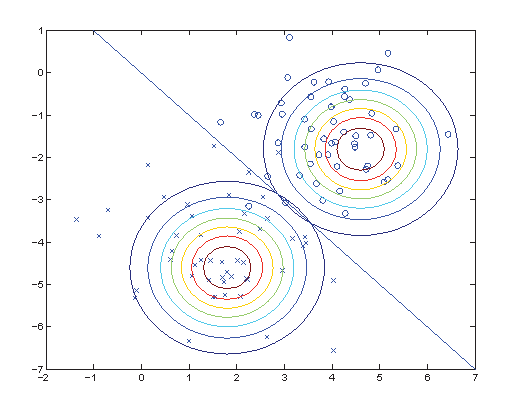
\includegraphics[width=0.6\textwidth]{GaussionOO.eps}
  \caption{高斯判别算法分类结果}
\end{figure}

\noindent分析:\\
直线两边的y值不同,但协方差矩阵相同,因此形状相同。$~\mu~$值不同,所以位置不同。

\subsubsection{GDA最大似然估计最佳参数详细推导}
\noindent对数似然函数:
\begin{equation}\nonumber
\begin{split}
  l(\phi,\mu_0,\mu_1,\Sigma)&=log\prod_{i=1}^{m}p(x^{(i)},y^{(i)})=log\prod_{i=1}^{m}p(x^{(i)}|y^{(i)})p(y^{(i)})=\sum_{i=1}^{m}log~p(x^{(i)}|y^{(i)})+log~p(y^{(i)})\\
                            &=\sum_{i=1}^{m}log~(p(x^{(i)}|y^{(i)}=0)^{1-y^{(i)}}\cdot p(x^{(i)}|y^{(i)}=1)^{y^{(i)}})+\sum_{i=1}^{m}log~p(y^{(i)})\\
                            &=\sum_{i=1}^{m}(1-y^{(i)})log~(p(x^{(i)}|y^{(i)}=0)+\sum_{i=1}^{m}y^{(i)}log~(p(x^{(i)}|y^{(i)}=1)+\sum_{i=1}^{m}log~p(y^{(i)})
\end{split}
\end{equation}
注意此函数分为三个部分,第一部分只与$~\mu_0~$有关;第二部分只与$~\mu_1~$有关;第三部分只$~\phi~$有关。最大化该函数,1.首先先求$~\phi~$,则求第一部分的偏导。
\begin{equation}\nonumber
\begin{split}
  \frac{\partial l(\phi,\mu_0,\mu_1,\Sigma)}{\partial\phi }&=\frac{\sum_{i=1}^{m}log~p(y^{(i)})}{\partial\phi}\\
   &=\frac{\partial\sum_{i=1}^{m}log~\phi^{y^{(i)}}(1-\phi)^{(1-y^{(i)})}}{\partial\phi}\\
   &=\frac{\partial\sum_{i=1}^{m}y^{(i)}log~\phi+(1-y^{(i)})log~(1-\phi)}{\partial\phi}\\
   &=\sum_{i=1}^{m}(y^{(i)}\frac{1}{\phi}-(1-y^{(i)})\frac{1}{1-\phi})\\
   &=\sum_{i=1}^{m}(I(y^{(1)}=1)\frac{1}{\phi}-I(y^{(i)}=0)\frac{1}{1-\phi})
\end{split}
\end{equation}
令其为零,求得$~\phi~$,(其中~I~是指示函数),
\begin{equation}\nonumber
\begin{split}
  {\color{red}{\phi=\frac{\sum_{i=1}^{m}I(y^{(i)}=1)}{m}}}
\end{split}
\end{equation}
2.同样地,对$~\mu_0~$求偏导,
\begin{equation}\nonumber
\begin{split}
  \frac{\partial l(\phi,\mu_0,\mu_1,\Sigma)}{\partial\mu_0}&=\frac{\partial\sum_{i=1}^{m}(1-y^{(i)})log~p(x^{(i)}|y^{(i)}=0)}{\partial\mu_0}\\
    &=\frac{\partial\sum_{i=1}^{m}(1-y^{(i)})(log\frac{1}{\sqrt{(2\pi)^2|\Sigma|}}-\frac{1}{2}(x^{(i)}-\mu_0)^T\Sigma^{-1}(x^{(i)}-\mu_0))}{\partial\mu_0}\\
    &=\sum_{i=1}^{m}(1-y^{(i)})\Sigma^{-1}(x^{(i)}-\mu_0)\\
    &=\sum_{i=1}^{m}I(y^{(i)}=0)\Sigma^{-1}(x^{(i)}-\mu)\\
\end{split}
\end{equation}
令其为0,得,
\begin{equation}\nonumber
\begin{split}
  {\textcolor{red}{\mu_0=\frac{\sum_{i=1}^{m}I\{y^{(i)}=0\}x^{(i)}}{\sum_{i=1}^{m}I\{y^{(i)}=0\}}}}\\
\end{split}
\end{equation}
3.同理得$~\mu_1~$,
\begin{equation}\nonumber
\begin{split}
  {\textcolor{red}{\mu_1=\frac{\sum_{i=1}^{m}I\{y^{(i)}=1\}x^{(i)}}{\sum_{i=1}^{m}I\{y^{(i)}=1\}}}}\\
\end{split}
\end{equation}
4.对$~\Sigma~$求偏导以求$~\Sigma~$(先改写初式前两部分),
\begin{equation}\nonumber
\begin{split}
  &\sum_{i=1}^{m}(1-y^{(i)})log~p(x^{(i)}|y^{(i)=0})+\sum_{i=1}^{m}y^{(i)}log~p(x^{(i)}|y^{(i)=1})\\
  =&\sum_{i=1}^{m}(1-y^{(i)})(log\frac{1}{\sqrt{(2\pi)^n|\Sigma|}}-\frac{1}{2}(x^{(i)}-\mu_0)^T\Sigma^{-1}(x^{(i)}-\mu_0))+\\
   &\sum_{i=1}^{m}y^{(i)}(log\frac{1}{\sqrt{(2\pi)^n|\Sigma|}}-\frac{1}{2}(x^{(i)}-\mu_1)^T\Sigma^{-1}(x^{(i)}-\mu_1))\\
  =& \sum_{i=1}^{m}log\frac{1}{\sqrt{(2\pi)^n|\Sigma|}}-\frac{1}{2}\sum_{i=1}^{m}(x^{(i)}-\mu_{y^{(i)}})^T\Sigma^{-1}(x^{(i)}-\mu_{y^{(i)}})\\
  =&\sum_{i=1}^{m}(-\frac{n}{2}log(2\pi)-\frac{1}{2}log(|\Sigma|))-\frac{1}{2}\sum_{i=1}^{m}(x^{(i)}-\mu_{y^{(i)}})^T(x^{(i)}-\mu_{y^{(i)}})
\end{split}
\end{equation}
进而有,
\begin{equation}\nonumber
\begin{split}
  \frac{\partial l(\phi,\mu_0,\mu_1,\Sigma)}{\partial\Sigma}&=-\frac{1}{2}\sum_{i=1}^{m}(\frac{1}{|\Sigma|}|\Sigma|\Sigma^{-1})-\frac{1}{2}\sum_{i=1}^{m}(x^{(i)}-\mu_{y^{(i)}})(x^{(i)}-\mu_{y^{(i)}})^T\frac{\partial\Sigma^{-1}}{\partial\Sigma}\\
  &=-\frac{m}{2}\Sigma^{-1}-\frac{1}{2}\sum_{i=1}^{m}(x^{(i)}-\mu_{y^{(i)}})(x^{(i)}-\mu_{y^{(i)}})^T(-\Sigma^{-2})\\
\end{split}
\end{equation}
这里用到的公式有,
\begin{equation}\nonumber
\begin{split}
  &\frac{\partial|\Sigma|}{\partial\Sigma}=|\Sigma|\Sigma^{-1}\\
  &\frac{\partial\Sigma^{-1}}{\partial\Sigma}=-\Sigma^{-2}\\
\end{split}
\end{equation}
令其为零,得,
\begin{equation}\nonumber
\begin{split}
  {\textcolor{red}{\Sigma=\frac{1}{m}\sum_{i=0}^{m}(x^{(i)}-\mu_{y^{(i)}})(x^{(i)}-\mu_{y^{(i)}})^T}}
\end{split}
\end{equation}

将参数全部求出后,可以看出公式推导相当复杂,但是结果是非常精简。
要判断一个新样本x时,可分别使用贝叶斯求出$~p(y=0|x)~$和$~p(y=1|x)~$,取概率更大的那个类。

实际计算时,我们只需要比大小,那么贝叶斯公式中分母项可以不计算,由于2个高斯函数协方差矩阵相同,则高斯分布前面那相同部分也可以忽略。实际上,GDA算法也是一个线性分类器,根据上面推导可以知道,GDA的分界线(面)的方程为:
\begin{equation}\nonumber
\begin{split}
  (1-\phi)exp((x-\mu_0)^T\Sigma{-1}(x-\mu_0))=\phi exp((x-\mu_1)^T\Sigma(x-\mu_1))
\end{split}
\end{equation}
取对数展开后化解,可得:
\begin{equation}\nonumber
\begin{split}
  2x^T\Sigma^{-1}(\mu_1-\mu_0)=\mu_1^T\Sigma^{-1}\mu_1-\mu_0^T\Sigma^{-1}\mu_0+log\phi-log(1-\phi)
\end{split}
\end{equation}
若,
\begin{equation}\nonumber
\begin{split}
  A&=2\Sigma^{-1}(\mu_1-\mu_0)=(a_1,a_2,\ldots,a_n)\\
  B&=\mu_1^T\Sigma^{-1}\mu_1-\mu_0^T\Sigma^{-1}\mu_0+log\phi-log(1-\phi)\\
\end{split}
\end{equation}
则,
\begin{equation}\nonumber
\begin{split}
  a_1x_1+a_2x_2+\ldots+a_nx_n=b
\end{split}
\end{equation}
这就是GDA算法的线性分界面。
\subsubsection{高斯判别分析与逻辑回归对比}
\noindent似然公式对比:\\
GDA:
\begin{equation}\nonumber
\begin{split}
  l(\phi,\mu_0,\mu_1,\Sigma)&=log\prod_{i=1}^{m}p(x^{(i)},y^{(i)};\phi,\mu_0,\mu_1,\Sigma)\\
  &=log\prod_{i=1}^{m}p(x^{(i)}|y^{(i)};\mu_0,\mu_1,\Sigma)p(y^{(i)};\phi)\\
\end{split}
\end{equation}
LR:
\begin{equation}\nonumber
\begin{split}
  L(\theta) &= p(\overrightarrow{y}|X;\theta)\\
            &= \prod_{i=1}^{m}p(y^{(i)}|x^{(i)};\theta)\\
            &= \prod_{i=1}^{m}(h_\theta(x^{(i)}))^{y^{(i)}}(1-h_\theta(x^{(i)})^{1-y^{(i)}}\\
  l(\theta) &= ln L(\theta)\\
            &= \sum_{i=1}^{m}y^{(i)}lnh(x^{(i)})+(1-y^{(i)})ln(1-h(x^{(i)}))
\end{split}
\end{equation}

\noindent结论一:\\
如果$~x|y~\sim~Gaussian~$即其服从正太分布,那么它的后验公式$~p(y=1|x)~$就是逻辑函数(sigmoid function)。\\
证明:\\
由贝叶斯公式可知:
\begin{equation}\nonumber
\begin{split}
  p(y=1|x)&=\frac{p(x|y=1)p(y=1)}{p(x)}\\
          &=\frac{N(\mu_1,\Sigma)\phi}{N(\mu_0,\Sigma)(1-\phi)+N(\mu_1,\Sigma)\phi}\\
          &=1/(1+\frac{N(\mu_0,\Sigma)}{N(\mu_1,\Sigma)}\frac{1-\phi}{\phi})\\
\end{split}
\end{equation}
而:
\begin{equation}\nonumber
\begin{split}
  \frac{N(\mu_0,\Sigma)}{N(\mu_1,\Sigma)}&=exp\{(x-\mu_0)^T\Sigma^{-1}(x-\mu_0)-(x-\mu_1)^T\Sigma^{-1}(x-\mu)\}\\
  &=exp\{2(\mu_1-\mu_0)^T\Sigma^{-1}x+(\mu_0^T\Sigma \mu_0-\mu_1^T\Sigma\mu_1)\}
\end{split}
\end{equation}
那么,令:
\begin{equation}\nonumber
\begin{split}
  &2\Sigma^{-1}(\mu_1-\mu_0)=(\theta_1,\theta_2,......,\theta_n)^T\\
  &\theta_0=\mu_0^T\Sigma\mu_0-\mu_1^T\Sigma\mu_1+log\frac{1-\phi}{\phi}
\end{split}
\end{equation}
则:
\begin{equation}\nonumber
\begin{split}
  p(y=1|x)=\frac{1}{1+exp(\theta_0+\theta_1x_1+\theta_2x_2+...+\theta_nx_n)}
\end{split}
\end{equation}
结论一得证。

\noindent结论二:\\
\begin{equation}\nonumber
\left\{
\begin{aligned}
\overset{.}x|y=1\sim Possion(\lambda_1) \\
x|y=0\sim Possion(\lambda_0)\\
\end{aligned}
\right.
\end{equation}
$$\Rightarrow p(y=1|x)\rightarrow logistic function.$$

在推导逻辑回归的时候,我们并没有假设类内样本是服从高斯分布的,因而GDA只是逻辑回归的一个特例,其建立在更强的假设条件下。故两者效果比较:\\
1.逻辑回归是基于弱假设推导的,则其效果更稳定,适用范围更广。\\
2.数据服从高斯分布时,GDA效果更好。\\
3.当训练样本数很大时,根据中心极限定理,数据将无限逼近于高斯分布,则此时GDA的表现效果会非常好。\\

\noindent\textbf{为何要假设两类内部高斯分布的协方差矩阵相同?}\\
从直观上讲,假设两个类的高斯分布协方差矩阵不同,会更加合理(在混合高斯模型中就是如此假设的),而且可推导出类似上面简洁的结果。\\
假定两个类有相同协方差矩阵,分析具有以下几点影响:\\
1.当样本不充分时,使用不同协方差矩阵会导致算法稳定性不够;过少的样本甚至导致协方差矩阵不可逆,那么GDA算法就没法进行\\
2.使用不同协方差矩阵,最终GDA的分界面不是线性的,同样也推导不出GDA的逻辑回归形式\\

\noindent\textbf{使用GDA时对训练样本有何要求?}\\
1.正负样本数的比例需要符合其先验概率。若是预先明确知道两类的先验概率,那么可使用此概率来代替GDA计算的先验概率;若是完全不知道,则可以公平地认为先验概率为50\%.\\
2.样本数必须不小于样本特征维数,否则会导致协方差矩阵不可逆,按照前面分析应该是多多益善。


\newpage
\section{回归}
回归是解决监督学习目标变量为连续值时,采用的学习方法。

回归,指研究一组随机变量$(Y_1,Y_2,\ldots,Y_i)$和另一组$(X_1,X_2,\ldots,X_k)$变量之间关系的统计分析方法,又称多重回归分析。通常$Y_1,Y_2,\ldots,Yi$是因变量,$X_1,X_2,\ldots,X_k$是自变量。

\subsection{线性回归}
线性回归的目的是寻找最佳拟合直线,做线性回归实战之前,要理解的东西有:线性函数是高斯分布在广义线性模型下建模;最小二乘法的概率解释;利用正规方程法求锝最佳回归系数;梯度下降法求得最佳回归系数。


\subsubsection{对高斯分布进行广义线性建模}
根据广义线性模型的形式化定义推导出高斯分布建模情况:\\
1.$~N(\mu,\sigma^2)\sim ExponentialFamily(\eta)$\\
2.令$~\sigma=1~$
\begin{equation}\nonumber
\begin{split}
  p(y;\mu)&=\frac{1}{\sqrt{2\pi}}exp(-\frac{1}{2})(y-\mu)^2\\
          &=\frac{1}{\sqrt{2\pi}}exp(-\frac{1}{2}y^2)\cdot exp(\mu y-\frac{1}{2} \mu ^2)
\end{split}
\end{equation}
对照指数分布族,得:
\begin{equation}\nonumber
\begin{split}
  \eta &= \mu\\
  T(y) &= y\\
  a(\eta)&=\mu^2/2\\
         &=\eta^2/2\\
  b(y)   &=(1/\sqrt{2\pi})exp(-y^2/2).\\
  ~\\
 So,~~~~~~ h(x) &=E(y|x)=\mu=\eta
\end{split}
\end{equation}
3.自然常数$~\eta~$与输入~X~是线性相关的,即:$~\eta = \theta x~$,\\
若$~\eta~$是向量,则$~\eta_i = \theta_i^T x.~$(我理解是预测多标签数据时的情况)。

\subsubsection{最小二乘法的概率解释:最大似然估计}
当我们面对回归问题时,为什么会采用线性回归,最小二乘法来定义成本函数,即1/2的差的平方和。
这里给出概率解释:\\
我们拟合的直线的函数值即预测值必然和真实值会存在误差。那么假定一个等式:\\
$$y^{(i)} = \theta^T x^{(i)}+ \epsilon^{(i)}$$
其中各个样本的误差项,是独立同分布且服从高斯分布(正态分布)。(可根据中心极限定理来看)\\
即就是:
$$\epsilon^{(i)} \sim N(0,\sigma^2)$$
$$P(\epsilon^{(i)})=\frac{1}{\sqrt{2\pi} \sigma}exp(-\frac{(\epsilon^{(i)})^2}{2 \sigma^2})$$
其$~\epsilon~$满足均值为0的正太分布易理解。因此:\\
$$P(y^{(i)}|x^{(i)};\theta)=\frac{1}{\sqrt{2\pi} \sigma}exp(- \frac{(y^{(i)}-\theta^Tx^{(i)})^2}{2\sigma^2}) $$
也就是要面对 在以为参数给定一个x时预测值y是真实值的概率服从正太分布,要求得概率最大时的?\\
则采用最大似然估计:
\begin{equation}\nonumber
\begin{split}
  L(\theta)&=\prod_{i=1}^{m}P(y^{(i)}|x^{(i)})\\
           &=\prod_{i=1}^{m}\frac{1}{\sqrt{2\pi} \sigma}exp(-\frac{(\epsilon^{(i)})^2}{2 \sigma^2})\\
~\\
  l(\theta)&=ln(L(\sigma))\\
           &=ln\prod_{i=1}^{m}\frac{1}{\sqrt{2\pi} \sigma}exp(-\frac{(\epsilon^{(i)})^2}{2 \sigma^2})\\
           &=\prod_{i=1}^{m}ln\frac{1}{\sqrt{2\pi} \sigma}exp(-\frac{(\epsilon^{(i)})^2}{2 \sigma^2})\\
           &=mln\frac{1}{\sqrt{2\pi}\sigma}-\frac{1}{\sigma^2}\cdot\frac{1}{2}\sum_{i=1}^{m}(y^{(i)}-\theta^Tx^{(i)})^2\\
\end{split}
\end{equation}
于是有:
\begin{equation}\nonumber
\begin{split}
           J(\theta)&=\frac{1}{\sigma^2}\cdot\frac{1}{2}\sum_{i=1}^{m}(y^{(i)}-\theta^Tx^{(i)})^2
\end{split}
\end{equation}
根据此过程,要求此$~L(\theta)~$函数的最大值 ,需求上式中后项函数的最小值$~J(\theta)~$,\\
函数$~J(\theta)~$又即为最小二乘估计的成本函数。\\
结论:上式推导即为最小二乘的概率解释。

\subsubsection{正规方程法找最佳回归系数}
\noindent\textbf{1.矩阵求导}\par
\begin{equation}\nonumber
\begin{split}
  \nabla_Af(A)=\left[\begin{array}{ccc}
\frac{\partial f}{\partial A_{11}}&\cdots&\frac{\partial f}{\partial A_{1n}}\\
\vdots&\ddots&\vdots\\
\frac{\partial f}{\partial A_{m1}}&\ldots&\frac{\partial f}{\partial A_{mn}}\\
\end{array}\right]
\end{split}
\end{equation}
函数自变量是矩阵,求导是对矩阵的每一个元素分别求导后,组成新的矩阵。\\
例:\\
\begin{equation}\nonumber
\begin{split}
 A &= \left[\begin{array}{cc}
    A_{11}&A_{12}\\
    A_{21}&A_{22}\\
              \end{array}\right]\\
f(A) &= \frac{2}{3} A_{11} +5 A_{12}^2 + A_{21}A_{22}\\
  \nabla_A f(A) &=\left[\begin{array}{cc}
  \frac{2}{3}&10A_{12}\\
  A_{22}&A_{21}\\
                        \end{array}\right]
\end{split}
\end{equation}

\noindent\textbf{2.矩阵的迹及常用性质与相关结论}\par
\noindent矩阵的迹:\\
$$trA=\sum_{i=1}^{m}A_{ii}$$
矩阵迹的常用性质:\\
\begin{equation}\nonumber
\begin{split}
&trABC = trCAB = trBCA\\
&trA = trA^T\\
&trA+B = trA +trB\\
&traA=atrA
\end{split}
\end{equation}
矩阵迹与矩阵求导相关结论:\\
\begin{align}
&\nabla_A trAB = B^T\\
&\nabla_{A^T}f(A) = (\nabla_Af(A))^T\\
&\nabla_A trABA^TC = CAB+C^TAB^T\\
&\nabla_A|A| = |A|(A^{-1})^T\\
&~\nonumber\\
combining ~&(2)~ and~ (3)~ :\nonumber\\
&\nabla_{A^T}trABA^TC = B^TA^TC^T+BA^TC
\end{align}

\noindent\textbf{3.利用正规方程求最佳回归系数}\par
\begin{equation}\nonumber
\begin{split}
input:&\\
X& = \left[\begin{array}{c}
    y^{(1)}\\
    y^{(2)}\\
    \vdots\\
    y^{(m)}\\
     \end{array}\right]\\
now:&\\
J(\theta)&=\frac{1}{2}(X\theta-\vec{y})^T (X\theta-\vec{y})\\
         &=\frac{1}{2}\sum_{i=1}^{m}(h_\theta(x^{(i)}-y^{(i)}))^2\\
Hence:&\\
\nabla_\theta J(\theta)&=\nabla_\theta\frac{1}{2}(X\theta-\vec{y})^T(X\theta-\vec{y})\\
                       &=\frac{1}{2}\nabla_\theta(\theta^TX^TX\theta-\theta^TX^T\vec{y}-\vec{y}^TX\theta+\vec{y}^T\vec{y})\\
                       &=\frac{1}{2}\nabla_\theta tr(\theta^TX^TX\theta-\theta^TX^T\vec{y}-\vec{y}^TX\theta+\vec{y}^T\vec{y})\\
                       &=\frac{1}{2}\nabla_\theta(tr\theta^TX^TX\theta-2tr\vec{y}^TX\theta)\\
                       &=\frac{1}{2}(X^TX\theta+X^TX\theta-2X^T\vec{y})\\
                       &=X^TX\theta-X^T\vec{y}=0\\
Normal~equations:&\\
X^TX\theta &=X^T\vec{y}\\
if~(X^TX)^{-1}~exist:&\\
\theta&=(X^TX)^{-1}X^T\vec{y}
\end{split}
\end{equation}

\subsubsection{实战:线性回归}
\noindent\textbf{1.利用线性回归寻找最佳拟合直线}\par
\noindent优点:结果易于理解,计算上不复杂。\\
缺点:对非线性的数据拟合不好。\\
适用数据类型:数值型和标称量型的数据。

实战是利用高斯分布广义线性建模出的连接函数,再利用最大似然估计得到最小二乘的成本函数。现,为得到最佳回归系数,有两种方式得到成本函数的最小值。\\
1.最优化算法。(梯度下降算法,牛顿法)\\
2.正规方程式。\\
两种方法各有千秋,最优化算法在训练集数量庞大时,优势便可以显现出来,因为其可以使用在线的最优化算法。而正规方程的方法,有严格的理论支持,若条件满足能得到最精确的最佳拟合直线,且不需要调参。、


用到的数学理论公式在上几节中都有记录:
\begin{equation}\nonumber
\begin{split}
 link~function~&:\\
 h(x) &=E(y|x)=\mu=\eta\\
 cost~function~&:\\
 J(\theta)&=\frac{1}{2}(X\theta-\vec{y})^T (X\theta-\vec{y})\\
         &=\frac{1}{2}\sum_{i=1}^{m}(h_\theta(x^{(i)}-y^{(i)}))^2\\
Normal~equations:&\\
X^TX\theta &=X^T\vec{y}\\
if~(X^TX)^{-1}~exist:&\\
\theta&=(X^TX)^{-1}X^T\vec{y}
\end{split}
\end{equation}

\noindent程序核心函数代码:
\begin{lstlisting}
def loadDataSet(fileName):      #general function to parse tab -delimited floats
    numFeat = len(open(fileName).readline().split('\t')) - 1 #get number of fields 2
    dataMat = []; labelMat = []
    fr = open(fileName)
    for line in fr.readlines():
        lineArr =[]
        curLine = line.strip().split('\t') #['1.000000', '0.116163', '3.129283']
        for i in range(numFeat):
            lineArr.append(float(curLine[i]))
        dataMat.append(lineArr)   #[[1.0, 0.52707], [1.0, 0.116163],...]
        labelMat.append(float(curLine[-1])) #[4.225236, 4.231083,...]
    return dataMat,labelMat

def standRegres(xArr,yArr):
    xMat = np.mat(xArr) #to matrix
    yMat = np.mat(yArr).T #to matrix with transform
    xTx = xMat.T*xMat  #xMat.T*xMat*w - xMat.T*yMat = 0
    if np.linalg.det(xTx) == 0.0:
        print ("This matrix is singular, cannot do inverse")
        return
    ws = xTx.I * (xMat.T*yMat)
    return ws


xArr,yArr = linear_regression.loadDataSet('ex0.txt') #feature matrix

ws = linear_regression.standRegres(xArr,yArr) #regression coefficient vector

#ouput : y = ws[0] + ws[1]*x
#drawing

xMat = np.mat(xArr)
yMat = np.mat(yArr)
yHat = xMat*ws      #prediction value

fig = plt.figure()
ax = fig.add_subplot(111)
ax.scatter(xMat[:,1].flatten().A[0],yMat.T[:,0].flatten().A[0],color='k')

xCopy = xMat.copy()
xCopy.sort(0) #sorted
yCHat = xCopy*ws

ax.plot(xCopy[:,1],yCHat,color='k')

plt.savefig('linear_fitting.eps',dpi=2000)
plt.show()

correlation_coefficient = np.corrcoef(yHat.T,yMat)
#1	0.986474
#0.986474	1
\end{lstlisting}

\noindent利用测试数据得到拟合直线,并可视化表示结果如下图:
\begin{figure}[!htb]
  \centering
  \includegraphics[width=0.6\textwidth]{2141.eps}
  \caption{线性回归得到拟合直线}
\end{figure}

\noindent分析:\par
任意数据集都可用线性进行建模,只是建模好坏有差异;程序中算得相关系数来计算预测值与真实值的匹配程度。\\
从拟合的效果图来看相当不错,但似乎有些欠拟合。该线性模型不能很好拟合出数据所存在的模式。

\noindent\textbf{2.利用局部加权线性回归寻找最佳拟合直线}\par
首先知道线性回归的一个问题就是欠拟合,将不能取得很好的预测效果。因为它是最小均方误差的无偏估计。
解决这一问题的方法就是允许估计中存在一些偏差。其中一个比较有效的方法就是局部加权线性回归(Locally Weighted Linear Regression)。\\
\noindent算法思想:\par
比较线性回归与局部加权线性回归:
\begin{equation}\nonumber
\begin{split}
LR&:\\
   &(1).Fit~\theta~to~minimize~\sum_{i=1}^{m}(y^{(i)}-\theta^Tx^{(i)})^2\\
   &(2).Output:~\theta^Tx\\
LWLR&:\\
   &(1).Fit~\theta~to~minimize~\sum_{i=1}^{m}w_{(i)}(y^{(i)}-\theta^Tx^{(i)})^2\\
   &(2).Output:~\theta^Tx\\
   &weighted:\\
   &w_{(i)}=exp(-\frac{(x_{(i)}-x)^2}{2\tau^2})
\end{split}
\end{equation}
解释:\\
当样本点$~x^{(i)}~$接近预测点x时,权值大。$~w^{(i)}\sim1~$.\\
当样本点$~x^{(i)}~$远离预测点x时,权值小。$~w^{(i)}\sim0~$.\\
权值系数$~w^{(i)}~$指数衰减,其中参数$~\tau~$为衰减因子,即权重衰减的速率。\\
$\tau~$越小 权重衰减越快。(依据权重函数易得知)\\
从后面实战中我们可以更好的理解参数$~\tau~.$ \\
\\
最小二乘法,求解最佳回归系数。
\begin{equation}\nonumber
\begin{split}
 J(\theta)&=\frac{1}{2}(X\theta-\vec{y})^TW(X\theta-\vec{y})\\
         &=\frac{1}{2}\sum_{i=1}^{m}w^{(i)}(h_\theta(x^{(i)}-y^{(i)}))^2\\
   weighted:&\\
   &w_{(i)}=exp(-\frac{(x_{(i)}-x)^2}{2\tau^2})\\
   order:&\\
   &\nabla_\theta J(\theta)=0\\
   \Rightarrow&~X^TWX\theta=X^TW\vec{y}\\
   \Rightarrow&~\theta=(X^TWX)^{-1}X^TW\vec{y}\\
\end{split}
\end{equation}

\noindent程序核心函数代码:
\begin{lstlisting}
def lwlr(testPoint,xArr,yArr,k=1.0):
    xMat = np.mat(xArr); yMat = np.mat(yArr).T
    m = np.shape(xMat)[0]
    weights = np.mat(np.eye((m)))
    for j in range(m):                      #next 2 lines create weights matrix
        diffMat = testPoint - xMat[j,:]   #difference matrix
        weights[j,j] = np.exp(diffMat*diffMat.T/(-2.0*k**2))   #weighted matrix
    xTx = xMat.T * (weights * xMat)
    if np.linalg.det(xTx) == 0.0:
        print ("This matrix is singular, cannot do inverse")
        return
    ws = xTx.I * (xMat.T * (weights * yMat))   #normal equation
    return testPoint * w
\end{lstlisting}

\noindent参数$~\tau~$的作用范围:
\begin{figure}[!h]
  \centering
  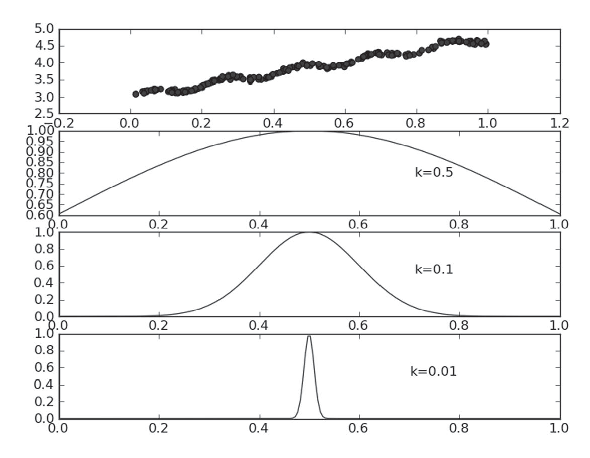
\includegraphics[width=0.55\textwidth]{tau.eps}
  \caption{$~\tau~$的作用范围}
\end{figure}

\noindent实验结果可视化:
\begin{figure}[!h]
  \centering
  \includegraphics[width=0.6\textwidth]{lwlr1.eps}
  \caption{$\tau=1$}
\end{figure}
\begin{figure}[!htb]
  \centering
  \includegraphics[width=0.6\textwidth]{lwlr0_01.eps}
  \caption{$\tau=0.01$}
\end{figure}
\begin{figure}[!htb]
  \centering
  \includegraphics[width=0.6\textwidth]{lwlr0_003.eps}
  \caption{$\tau=0.003$}
\end{figure}\\
分析:\\
从结果来看 局部线性回归能很好地解决线性回归欠拟合的问题,但又可能出现过拟合。\\
所以参数调整影响了模型的泛化能力。选取合适参数至关重要。\\
虽然局部线性回归能增强模型的泛化能力。但是它也有自己的缺陷。就是对每个点的预测都必须使用整个数据集。这样大大增加了计算量。\\

\noindent存在问题:\\
考虑一个问题,当数据特征比训练集样本点还多时,也就是说不可逆,矩阵求导无计可施。此时就要用缩减样本来“理解”数据,求得回归系数矩阵。
即就是:
\begin{equation}\nonumber
\begin{split}
  &R(X^TX)=R(X)=m\\
  &if~\#feature>\#sample ~~(n>m)\\
  &X^TX\in R^{n\times n}\\
  So,&(X^TX)^{-1}~not~exist.
\end{split}
\end{equation}

\noindent\textbf{3.预测鲍鱼年龄}\par
\noindent实战代码以及结果见注释:\\
\noindent程序核心函数代码:
\begin{lstlisting}
def standRegres(xArr,yArr):
    xMat = np.mat(xArr)
    yMat = np.mat(yArr).T
    xTx = xMat.T*xMat  #xMat.T*xMat*w - xMat.T*yMat = 0
    if np.linalg.det(xTx) == 0.0:
        print ("This matrix is singular, cannot do inverse")
        return
    ws = xTx.I * (xMat.T*yMat)
    return ws

def lwlr(testPoint,xArr,yArr,k=1.0):
    xMat = np.mat(xArr); yMat = np.mat(yArr).T
    m = np.shape(xMat)[0]
    weights = np.mat(np.eye((m)))
    for j in range(m):                      #next 2 lines create weights matrix
        diffMat = testPoint - xMat[j,:]   #difference matrix
        weights[j,j] = np.exp(diffMat*diffMat.T/(-2.0*k**2))   #weighted matrix
    xTx = xMat.T * (weights * xMat)
    if np.linalg.det(xTx) == 0.0:
        print ("This matrix is singular, cannot do inverse")
        return
    ws = xTx.I * (xMat.T * (weights * yMat))   #normal equation
    #ws #7 feature,and 1
    return testPoint * ws

#locally weighted linear regression
yHat01 = function.lwlrTest(abX[0:99],abX[0:99],abY[0:99],0.1) #training set #0-99
yHat1 = function.lwlrTest(abX[0:99],abX[0:99],abY[0:99],1)
yHat10 = function.lwlrTest(abX[0:99],abX[0:99],abY[0:99],10)

#error
error01 = function.rssError(abY[0:99],yHat01.T)   #56.820227823572182
error1 = function.rssError(abY[0:99],yHat1.T)   #429.89056187016683
error10 = function.rssError(abY[0:99],yHat10.T)   #549.1181708825128

#generalization
yHat01g = function.lwlrTest(abX[100:199],abX[100:199],abY[100:199],0.1) #test set #100-199
yHat1g = function.lwlrTest(abX[100:199],abX[100:199],abY[100:199],1)
yHat10g = function.lwlrTest(abX[100:199],abX[100:199],abY[100:199],10)

#error
error01g = function.rssError(abY[100:199],yHat01g.T)   #36199.797699875046
error1g = function.rssError(abY[100:199],yHat1g.T)   #231.81344796874004
error10g = function.rssError(abY[100:199],yHat10g.T)   #291.87996390562728

#compare
#k = 0.1 overfitting

#linear regression
ws = function.standRegres(abX[0:99],abY[0:99])
yHat = np.mat(abX[100:199])*ws
errorlr = function.rssError(yHat.T.A,abY[100:199])   #518.63631532510897

#compare
#lwlr is better than lr
\end{lstlisting}

%\subsection{缩减系数来理解数据}